% !TEX TS-program = pdflatex
% !TEX encoding = UTF-8 Unicode

% This is a simple template for a LaTeX document using the "article" class.
% See "book", "report", "letter" for other types of document.
\documentclass[11pt]{article} % use larger type; default would be 10pt
\usepackage[utf8]{inputenc} % set input encoding (not needed with XeLaTeX)

% These packages are optional, depending whether you want the features they provide.

%%% PAGE DIMENSIONS
\usepackage{geometry} % to change the page dimensions
\geometry{letterpaper} % or letterpaper (US) or a5paper or....
\geometry{margin=1in} % for example, change the margins to 2 inches all round
% \geometry{landscape} % set up the page for landscape

\usepackage{graphicx} % support the \includegraphics command and options
\usepackage{hyperref}

\usepackage[parfill]{parskip} % Activate to begin paragraphs with an empty line rather than an indent

%%% PACKAGES
%\usepackage{booktabs} % for much better looking tables
\usepackage{array} % for better arrays (eg matrices) in maths
%\usepackage{paralist} % very flexible & customisable lists (eg. enumerate/itemize, etc.)
\usepackage{verbatim} % adds environment for commenting out blocks of text & for better verbatim
%\usepackage{subfig} % make it possible to include more than one captioned figure/table in a single float

%%% HEADERS & FOOTERS
\usepackage{fancyhdr} % This should be set AFTER setting up the page geometry
\pagestyle{fancy} % options: empty , plain , fancy
\renewcommand{\headrulewidth}{0pt} % customise the layout...
\lhead{}\chead{}\rhead{}
\lfoot{}\cfoot{\thepage}\rfoot{}

%begin the doc

\title{Introduction to Microcontrollers: Exploring Interfaces}
\author{}
\date{} % Activate to display a given date or no date (if empty),

\begin{document}
\maketitle

\section*{Introduction}
...
%At this point, we have seen simple examples of how to measure something about our surroundings using an oscilloscope  (e.g., temperature) and how to change something (e.g., using a heater to warm up our enclosures).  But all of these experiments were done `manually' -- you turned on a voltage supply or read the temperature from a data stream. What we're missing is \emph{control}.
test
With the proliferation of modern microcontrollers, control of electromechanical systems has moved from dedicated circuitry and specialized hardware to more general implementations where a small computer -- the microcontroller -- is programmed to work with various sensors and actuators using high-level languages (e.g., C or BASIC). One of the primary benefits is that microcontrollers are very flexible, and that flexibility allows the designer to quickly change parameters and try them out without having to significantly redesign the system hardware (think prototyping!).

In this lab, you’ll explore different ways to get information from a sensor into the microcontroller and perform some basic processing. Specifically, you’ll determine whether or not light is hitting a photoresistor and use it to make a simple night light. You’ll also use the oscilloscope to probe the circuit so you can learn more about its functionality.

\subsection*{Objectives}

Upon completion of this lab, the student should be able to:
\begin{itemize}
\item Program an Arduino to perform digital input and output,
\item Program an Arduino to perform basic control and logical functions,
\item Demonstrate an understanding of an RC circuit,
\item Use an oscilloscope to observe the dynamic response of an electronic circuit, and 
\item Use a comparator to add precision to a sensor reading.

\end{itemize}

\section*{Preparation}

\begin{description}
\item [Basic laws of capacitors and RC circuits.] Review RC circuits from your Physics classes. Read Carryer \emph{et al.}, Sections 9.6 up to and including 9.9.2. Pay particular attention to anything related to RC circuits in the time domain. Read the rest of Section 9.9 if you want. Read 9.14 on real capacitors, if you're interested.
%\item [If you want more on RC circuits.] Watch the video on collab under Resources. Note that it was originally geared specifically towards low-pass filters, but the analysis is the same for our needs here.
\end{description}
{\bf You must complete the pre-lab worksheet before you come to lab.} The worksheet is an individual assignment.

\subsection*{Analog vs. Digital}

%When we speak of things being \emph{analog}, we mean that they can take on any value in a continuous range. A bicycle can travel at any speed between zero and whatever the cyclist's top speed is.\footnote{Your professor has topped out at 85 km/h going down a mountain pass.} The outdoor temperature can take on any value between ``deep-freeze'' and ``scorching''. The voltage across a resistor can be any value. Most of the world is indeed analog.
%
%In contrast, something that is \emph{digital} can take on one of two values: A light switch is either ON or OFF. A door is locked or unlocked. Likewise, computers and microcontrollers, which are really just complicated sets of switches, can only represent discrete values. Indeed, except for all but the most specialized computers, deep down, they can really only represent two values: `1' and `0'. Of course, these 1's and 0's can be arranged to represent a discrete range of values so the question is, how do we get from the analog world to a digital representation of the world in a microcontroller...and vice versa?
%
%Before we tackle that, let's take a step back. \emph{Sometimes} all we care about is digital information: it might not matter what the temperature in your house is, but if it's too cold, the furnace should come on. When the furnace comes on, it is generally either ON or OFF, not ``3/4 ON'' or “HALF OFF”. In these cases, the relevant information is digital. 

To begin with, we’ll recap digital and analog interfaces. There are four potential kinds of connections between a microcontroller and the outside world: digital in, digital out, analog in, and analog out. Physically, these interfaces are through wires, called \emph{pins} on the microcontroller, and each pin is addressed through internal circuitry, which sets or reads \emph{voltages} at the pins, based on whatever program has been put on the microcontroller by a programmer.


\begin{itemize}
\item \emph{Digital output} is probably the easiest of the interfaces. Digital output can either be LOW, in which case the output pin is connected to ground (0V) via internal circuitry, or HIGH, in which case the pin is connected to whatever the supply voltage is (5V, in your system). In Arduino, digital output is accomplished by setting the pin as an output with \verb|pinMode()| and then using \verb|digitalWrite()| to set the pin HIGH or LOW. Note that if you pass enough current through a pin, the voltage might differ from 0 V or 5 V by a few tenths of a volt.
\item Perhaps surprisingly, \emph{digital input} is a little more complex than digital output. The reason is that there is no guarantee that the voltage applied externally to a pin will be exactly 0V or 5V. The circuitry must tolerate variances from defined HIGH and LOW voltages, leaving a gray area where the reading is ambiguous. In Arduino, reading a digital value is accomplished by setting the pin as an input with \verb|pinMode()|\footnote{When a program is started, all of the digital pins default to input pins, though it is still a good idea to declare them as such, just for clarity.} and reading it with verb|digitalRead()|.
\item \emph{Analog input} is generally accomplished by means of an \emph{analog-to-digital converter}, or simply, an \emph{ADC}. An ADC takes a continuous range of voltages and divides it up into a discrete set of numbers, where the size and range depends on the specifics of the ADC. The conversion formula has been covered elsewhere. Reading an analog pin is accomplished using \verb|analogRead()|.
\item \emph{Analog output} is probably the most complicated of the interfaces. In fact, it's complicated enough at the hardware level that with the Arduino Uno, analog output isn't analog at all -- it's digital! Essentially, internal timers switch the voltage back and forth between HIGH and LOW at a very high rate such that the \emph{average} voltage approximates the desired analog voltage. We’ll cover this method, called \emph{pulse width modulation} (PWM) later in the term.
\end{itemize}

\section*{In lab}

Lab activities will center around making a night light. Although not the most advanced system you can make, it allows us to explore a lot of the functionality of a microcontroller.

\subsection*{Night light with an ADC}

Here, you’ll use the analog-to-digital converter again to determine if it is dark (and the night light is needed) or light.

\subsubsection*{Procedure}

You will use this circuit for several experiments today, so be sure to place it in a convenient spot on your breadboard.

\begin{enumerate}
\item Begin building circuits in Figure~\ref{fig:night.light}. When you insert the photoresistor into your breadboard, put it about 3-4 cm from the LED, but don’t connect it to the resistor, $R$, just yet. Gently, bend it and the white LED so that they face each other -- you’ll want them close enough to get a good signal while still being able to pass a pencil or a finger between them without bumping either. Once you’ve arranged them, try not to bump either component so that the measurements you are about to take will consistent for the rest of the lab.
\item Using jumper wires (so you don’t disturb the photoresistor) and a DMM, measure and record the resistance of the photoresistor when the LED is on and when it is off. This will correspond to “day” and “night” for your nightlight.

\begin{figure}[htbp]
\begin{center}
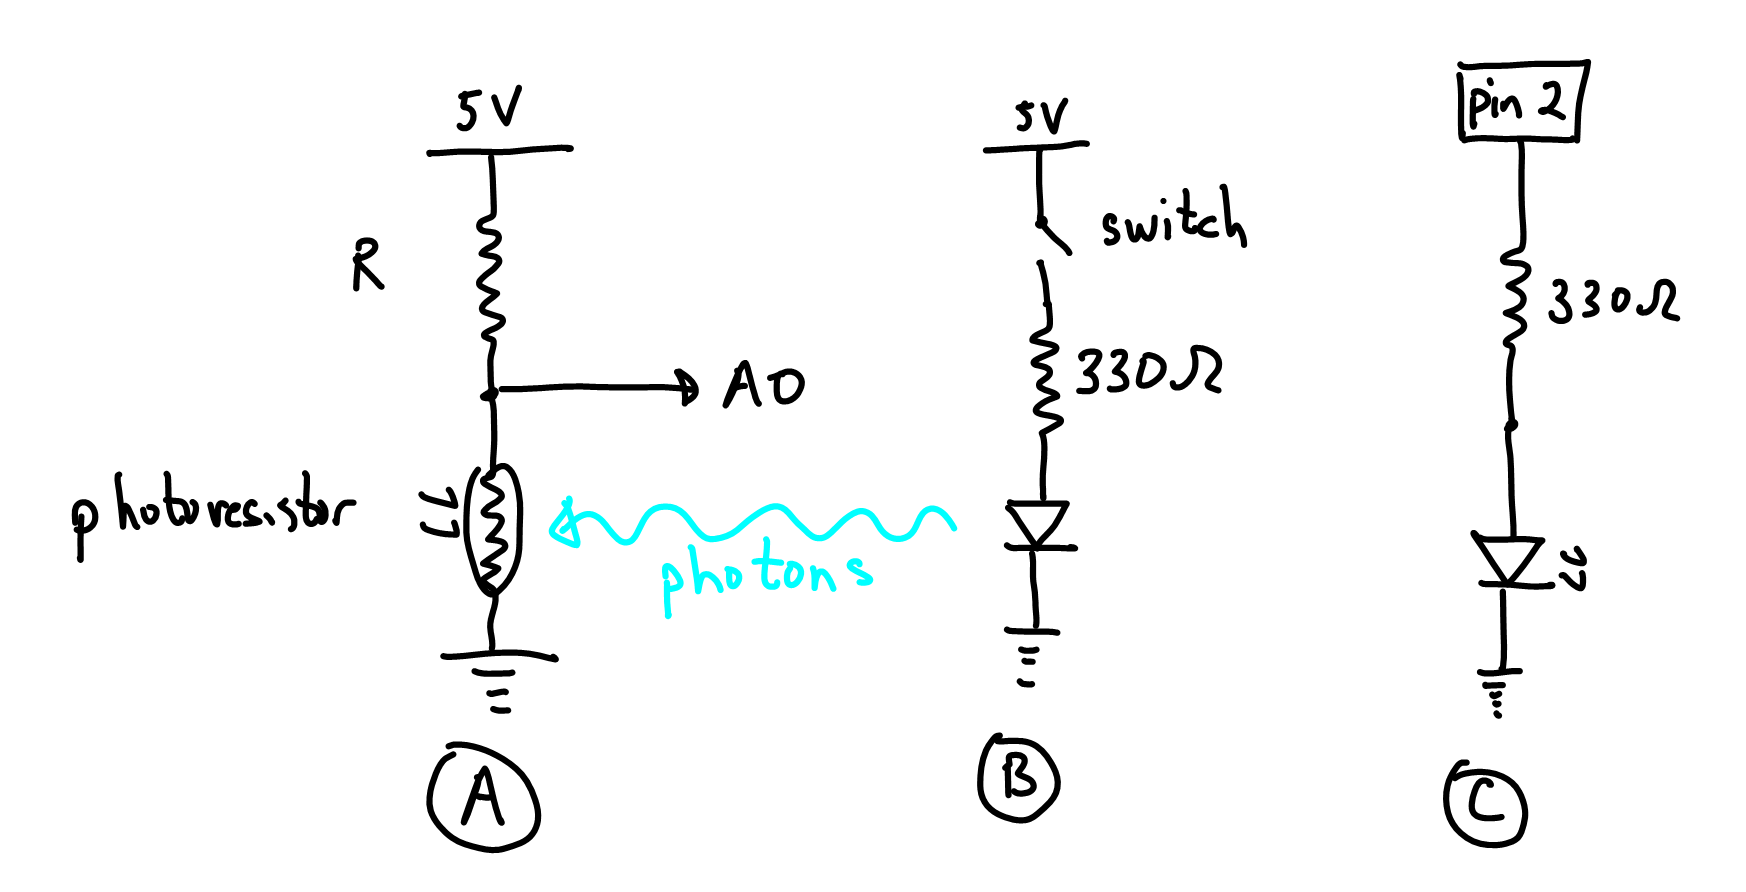
\includegraphics[width=\textwidth]{figures/night_light}
\caption{Circuits for the night light. Circuit A is the photosensor; B is a manually controlled LED to make it “day” or “night”; C is the night light, which you’ll control from pin 2.}
\label{fig:night.light}
\end{center}
\end{figure}

\vspace{0.25in}
Resistance (day): \rule{2in}{0.4pt}

\vspace{0.25in}
Resistance (night): \rule{2in}{0.4pt}
\vspace{0.25in}

\item Choose a fixed resistor, $R$, with a value that is near the geometric mean of the two values you measured before and insert into the circuit. It can be shown that doing so will give the largest voltage swing at the junction.
\item Write a program that uses the ADC to read the voltage at the junction every 500 ms. Print the state (“light” or “dark”) to the Serial Monitor and turn the “night light” on or off appropriately. That is, you’ll have to find a useful threshold and write the logic to turn the light on and off.
\end{enumerate}

{\bf Demonstrate your working system to an instructor.}

\subsection*{Basic RC circuit}
\label{sec:rc.circuit}

In the above example, the light intensity is clearly an \emph{analog} value. Given such a problem, it’s quite common to use the ADC to measure voltages, but it’s not the only way. In this next experiment, you’ll use an RC-circuit to measure changes in resistance. Such a technique is invaluable to measure changes in \emph{capacitance} if you happened to have a capacitance-based sensor.

First, you’ll analyze a basic RC-circuit, then you’ll put the theory to use to measure light levels.

\subsubsection*{Procedure}

\begin{enumerate}
\item You’ve been provided a nominal $1000\Omega$ resistor and a $0.1\mu F$ capacitor. Use a DMM to measure the actual resistance and capacitance of the components and calculate the rise time for the circuit in Figure~\ref{fig:rc.circuit}. Also calculate the time-constant.

\vspace{0.25in}
Calculated rise-time ($10\rightarrow 90\%$): \rule{2in}{0.4pt}

\vspace{0.25in}
Calculated time-constant: \rule{2in}{0.4pt}
\vspace{0.25in}

\item Without disturbing your existing circuits, construct the circuit in Figure~\ref{fig:rc.circuit}. The circuit will be driven by a digital output pin. We'll use the oscilloscope to simultaneously measure the input voltage on CH1 and the output voltage between the resistor and capacitor on CH2.
\begin{figure}[h]
\centering
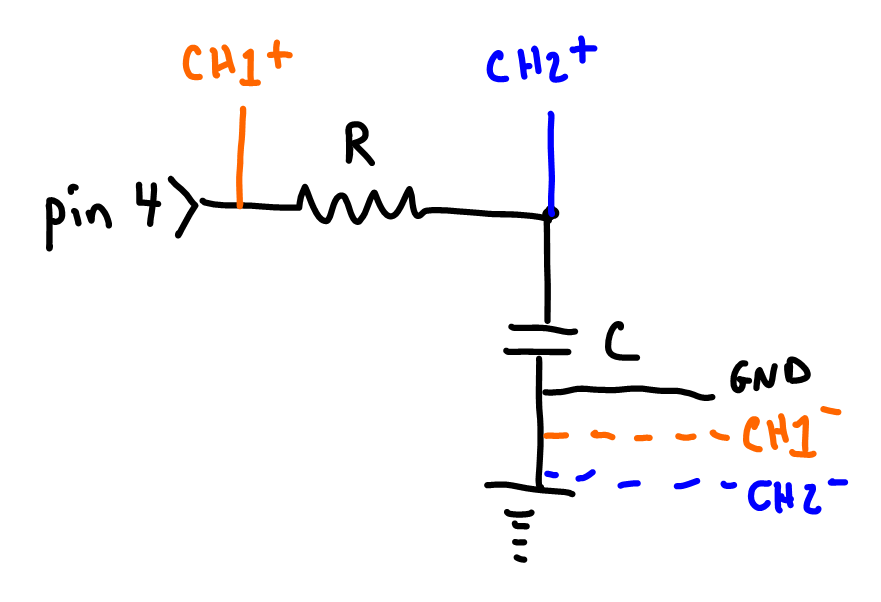
\includegraphics[width=0.4\textwidth ]{figures/RC_circuit_digilent.png}
%\end{center}
\caption{RC circuit with connections to the Analog Discovery labelled. GND here refers to the black wire on the Analog Discovery (denoted by an arrow on the device). Connect the GND from the Arduino as normal.}
\label{fig:rc.circuit}
\end{figure}

\item Write a program that sets pin 4 as an OUTPUT and toggles the state between HIGH and LOW every 1 ms. Use \verb|delay()| to perform the timing. Check that you won’t exceed the current limits of an output pin.
%\item Set AWG1 to produce a square wave that jumps back and forth between 0V (LOW) and and 5V (HIGH). Set the period to be substantially larger than the rise-time you calculated for this circuit in the pre-lab; 5-10 times greater is a reasonable amount; Basically, you want the the output voltage to reach the input voltage before the latter jumps again.
\item In the Waveforms software, run the oscilloscope and set the trigger to Normal. Adjust the settings to capture a rising signal on CH1 with a threshold of 2V.
\item Explore the functionality of the Waveforms software by adjusting the timescale and offsets. Note how you can adjust the various levels by grabbing the appropriate triangle and dragging it. One thing you will probably want to do is go to Options $\rightarrow$ Display and change the offsets for both Voltage and Time to ``Divisions.'' This will prevent the draggable triangles from disappearing when you drastically change the scales.
\item Adjust the oscilloscope settings so that you have a good view of the voltage on CH2. Eyeball the rise-time. Does it look reasonable, given your calculations? If not, check your connections and re-calculate the rise-time from the pre-lab. Small variations are normal; being off by an order of magnitude indicates something is wrong.
\item In the oscilloscope program, find the ``Measure'' option and explore the built-in measurements provided in the software. Dig around until you find ``Rise Time'' and add the measurement (for the channel connected to the output) to your list of measurements. How does the measured rise-time compare to your calculations? Give possible explanations for any discrepancies.

\vspace{0.25in}
Measured rise-time: \rule{2in}{0.4pt}
\vspace{0.25in}

\item Set the trigger to capture on the falling edge and calculate the fall-time. Is it different from the rise-time? Explain.
\item Change the trigger to CH2. Grab the trigger level triangle and drag it up and down a little. What happens?
%\item Capture a couple cycles of both the input and output and {\bf save them for the Numerical Simulation lab you will start in the post processing section!}
\end{enumerate}

\subsection*{The RC timer}

When you measured the rise and fall time of the RC-circuit in Section~\ref{sec:rc.circuit}, the circuit had two essential connections: an input (the Arduino pin and CH1) and an output (CH2). The circuit in Figure~\ref{fig:rc.photoresistor}, however, uses only one connection, but the math is essentially the same as the previous circuit. In this circuit, the Arduino pin will both charge the capacitor \emph{and} measure its decay. To charge the capacitor, you need to set the pin to be an output and turn it HIGH. But you can't just turn it LOW to time the decay -- it would immediately source all the current and drain the capacitor. Instead, you must switch it to be an INPUT pin, which will allow you to monitor the voltage without sinking any current. The $100\Omega$ resistor is simply acting as a current limiter during the charging phase -- during the decay, the Arduino pin is set as an input and already has a very large resistance, so the small extra resistance is irrelevant.

%\begin{figure}
%\centering
%\includegraphics[width=2in]{figures/RC_timer.png}
%\caption{An RC-circuit configured as an RC timer.}
%\label{fig:rc.timer.circuit}
%\end{figure}

\subsubsection*{Procedure}

\begin{enumerate}
\item Leaving the photoresistor in place, remove all of the other components from Circuit A in Figure~\ref{fig:night.light}.
\item Replace it with the circuit in Figure~\ref{fig:rc.photoresistor}. 

\begin{figure}
\centering
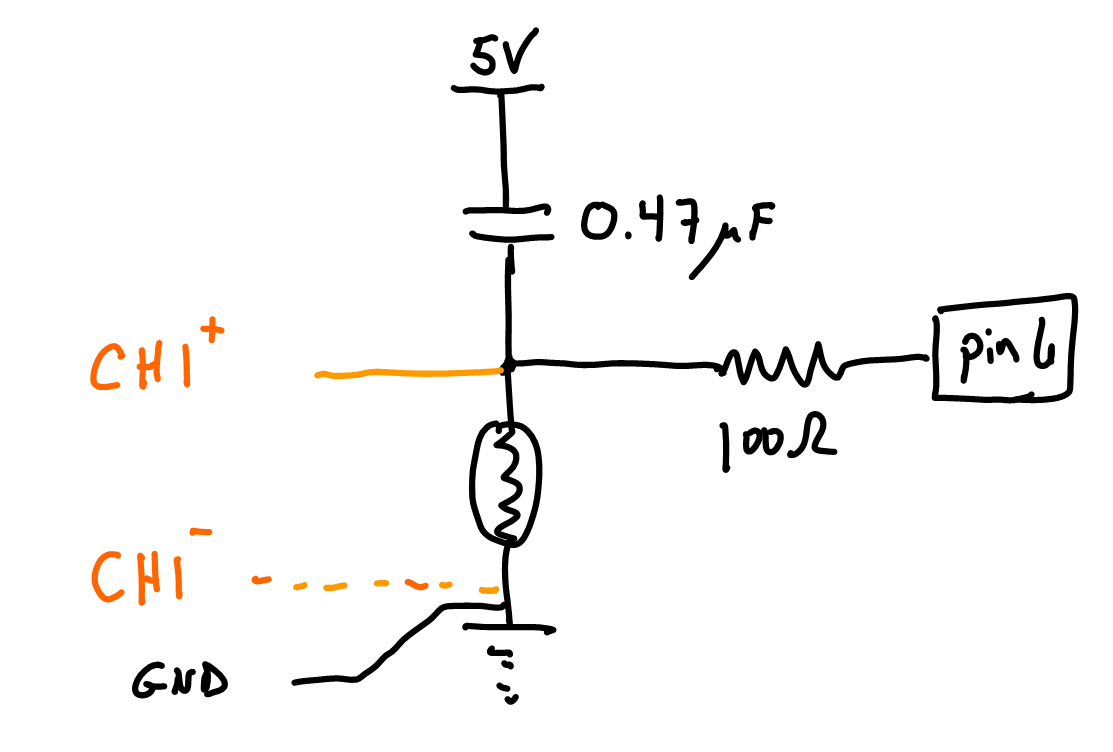
\includegraphics[width=3in]{figures/RC_photoresistor.png}
\caption{An RC-timer with a photoresistor as the resistive element.}
\label{fig:rc.photoresistor}
\end{figure}

\item Add a \emph{function} that reads the decay time of the RC circuit, as follows:
\begin{enumerate}
\item Set pin 7 as an OUTPUT.
\item Set the pin to HIGH.
\item Wait 2ms for the capacitor to charge. Use \verb|delay()|.
\item Set the pin as an INPUT.
\item Record the start time using \verb|micros()|.
\item Wait for the pin to go LOW.
\item Record the end time using \verb|micros()|.
\item Return the difference between the two times -- i.e., the decay time.
\end{enumerate}
\item Use CH1 on the oscilloscope to measure the voltage across the photoresistor, as shown.
\item Starting with the LED toggling program, edit it so that it calls the new function in the program’s \verb|loop()| and writes the decay time to the Serial Monitor every 1 s. For now, just continue to use a \verb|delay()| function to slow the loop down.
\item Run the program and toggle the light on and off. Note the decay time and compare it to the fall time read by the oscilloscope. Record both values in Table~\ref{tab:rc.dynamics}. Why aren’t they the same? Do they show the same trends?

\begin{table}[htp]
\begin{center}
\begin{tabular}{|c|c|c|}
 & Fall time & Decay time \\
Condition & (measured from oscilloscope) & (measured by the Arduino)\\
 \hline
Light & &\\
Dark & &\\
\end{tabular}
\end{center}
\caption{RC timer dynamics}
\label{tab:rc.dynamics}
\end{table}%

\end{enumerate}

{\bf Demonstrate your working system to an instructor.}

\subsection*{Precision timing with a comparator}

Though easy to implement, the RC-timer above suffers from one potential pitfall, namely that you are not guaranteed that the pin on the ATmega328 will switch from \verb!HIGH! to \verb|LOW| at a consistent voltage. That is, the datasheet guarantees that any voltage below 1 V will register as \verb|LOW| and anything above 3V as \verb|HIGH|. In between, the pin state is undefined, and while it may switch at a consistent value for this lab, there’s no guarantee that it will continue to do so, especially when more components are added to the system. For this system, it’s hardly critical, but in others, it is necessary to define a precise threshold for the RC-timer.

A straightforward solution to the dilemma is to use a \emph{comparator} to set a precise threshold where the pin will change, as shown in Figure~\ref{fig:comparator.rc}. A comparator does just as its name suggests: it compares two voltages and outputs a \verb|HIGH| or \verb|LOW| depending on which is higher: if the input on the \emph{non-inverting} input (labelled with a ‘\verb|+|’) is higher than the \emph{inverting} input (with a ‘\verb|-|’), it outputs a \verb|HIGH|; otherwise it outputs a \verb|LOW|. Thus, one can establish the threshold voltage for the RC decay using a voltage divider and use the comparator to precisely time the decay. The added precision comes at a cost, however. Not only do you need an extra component, but you must also use two pins on the Arduino since you can’t send current “backwards” through the comparator, you’d need one pin to read the compartor and a second pin to charge the capacitor.

\begin{figure}[htbp]
\begin{center}
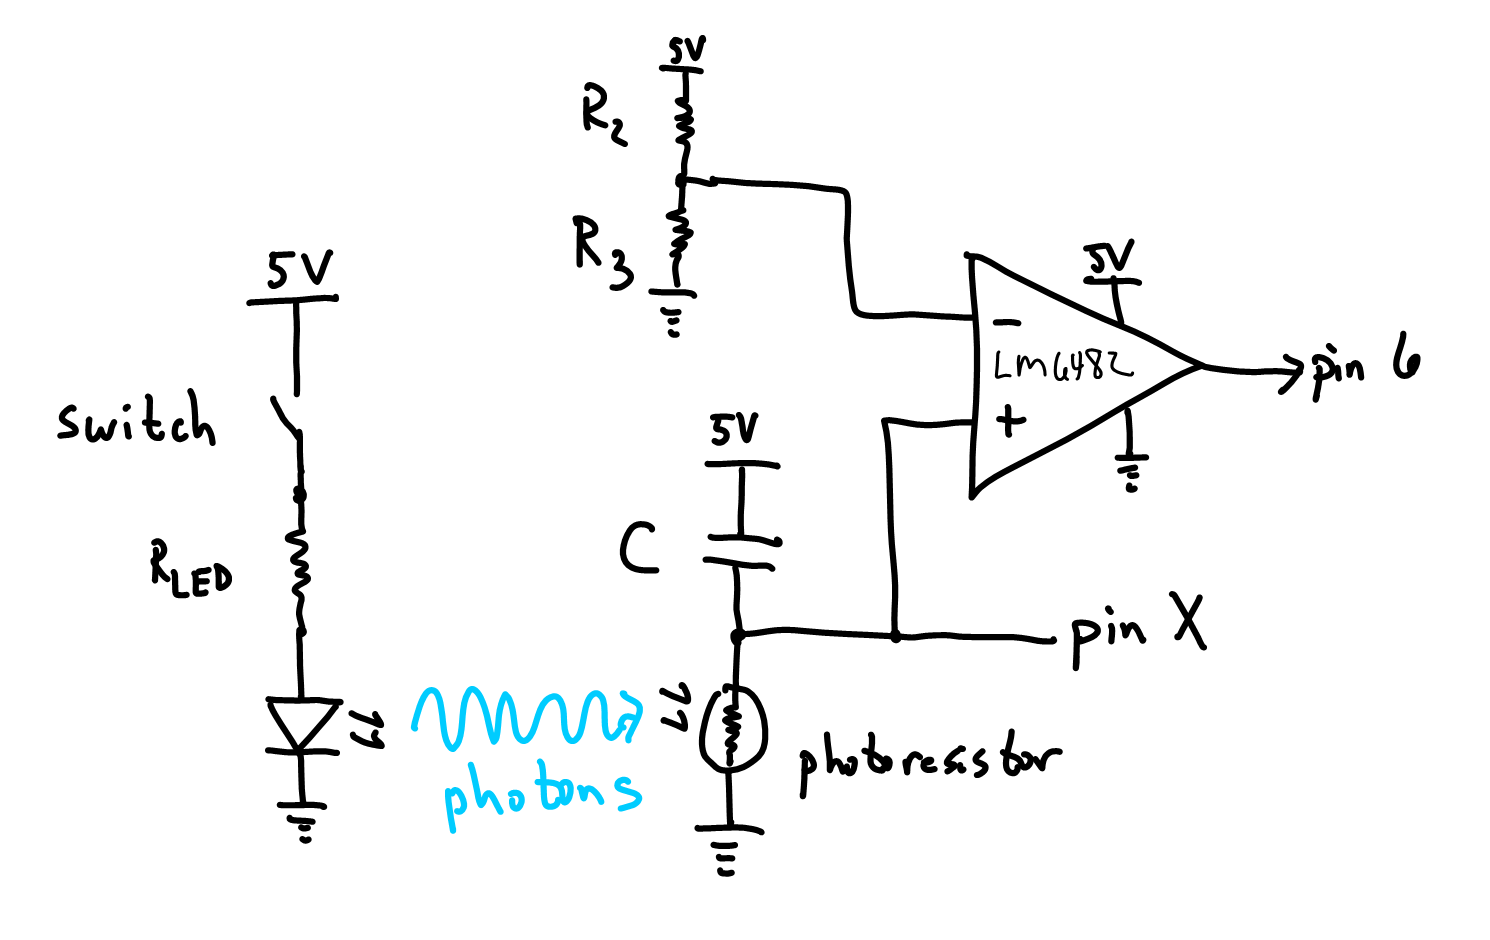
\includegraphics[width=4in]{figures/comp_rc}
\caption{Circuit for precision timing using an external comparator. \emph{Do not build this circuit} -- there is an easier way!}
\label{fig:comparator.rc}
\end{center}
\end{figure}

The circuit can be simplified greatly by using the built-in comparator on the ATmega328. By default, pins 6 and 7 on the Arduino (\verb|PIND6| and \verb|PIND7| on the ATmega328) are the non-inverting (\verb|AIN0|) and inverting (\verb|AIN1|) terminals, respectively, of an internal comparator. Unlike a dedicated op-amp, the comparator does not have an output pin, but instead controls an internal value that can be read with a low-level commands:

\begin{verbatim}
  int comparatorOutput = (ACSR >> ACO) & 0x01;
\end{verbatim}

A little arcane, but \verb|comparatorOutput| in the line above will be \verb|1| when the voltage on pin 6 is greater than pin 7 and \verb|0| otherwise. The nice part is that you can freely command the pins to be inputs or outputs without worrying about the comparator -- it runs in the background regardless.

\begin{enumerate}
\item Build the circuit in Figure~\ref{fig:comp.internal}. The resistors in the voltage divider on pin 7, the inverting terminal of the comparator, should be sized to create as close to 1.84V as reasonable. (Why did I choose 1.84V?) A good rule-of-thumb is to make the series resistance somewhere between $10k\Omega - 50k\Omega$.

\begin{figure}[htbp]
\begin{center}
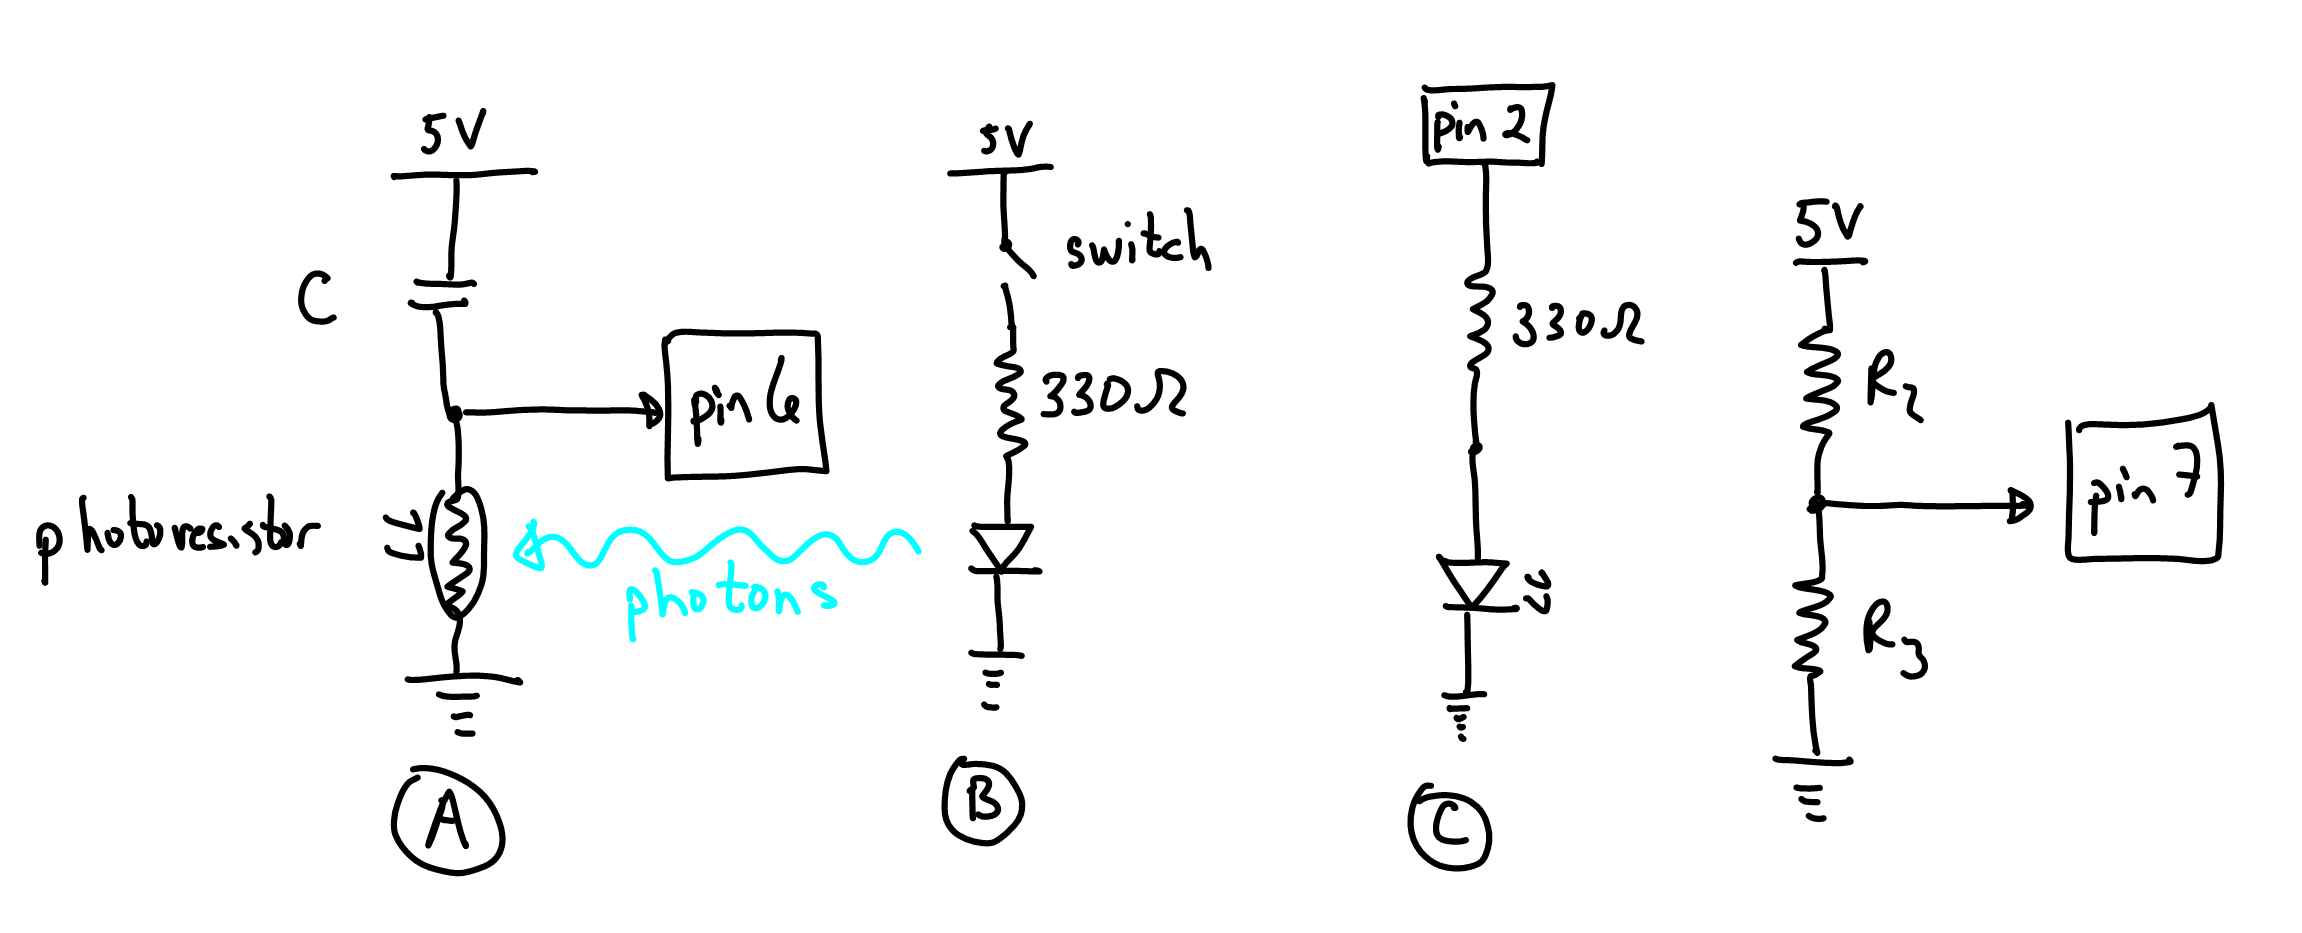
\includegraphics[width=\textwidth]{figures/comp_internal}
\caption{Circuit for precision timing using the ATmega328’s internal comparator. It is much easier than the external comparator above.}
\label{fig:comp.internal}
\end{center}
\end{figure}

\item Edit your code from the previous section to read the output of the internal comparator, instead of the pin directly.
\item Run your code again and use your oscilloscope to confirm that the decay time is the same as before.
\end{enumerate}

{\bf Demonstrate your working system to an instructor.}

%\section*{Design Challenge}
%
%{\bf Due at the end of lab.} Build a motion activated night light, with the following functionality:
%
%\begin{itemize}
%\item When it is dark AND there is motion detected, an LED is lit and stays on for 10 seconds \emph{after the last motion stops}.
%\item Otherwise (i.e., light or no motion), the LED doesn’t come on.
%\item You will use your white LED for the night light.
%%\item You must use a software timer object (as discussed in class) for the timer. 
%%\item If the ambient light comes on before the 10 seconds is up, the night light will turn off.
%%\item You may register light or dark with any method that uses a comparator (hint: the easiest way is the one permutation you did not use above), but \emph{you must use ambient light} as the light source. You may create darkness by covering the photoresistor, turning off the lights, dementors, or whatever it takes (except altering your circuit).
%\end{itemize}
%
%{\bf You must demonstrate your working system to an instructor.} If you do not finish in lab, expect to demonstrate it before or after class on Friday.
%
%\vspace{0.25in}
%Instructor sign-off: \rule{2in}{0.4pt}
%\vspace{0.25in}
%


%\subsection{Putting it all together}
%
%{\bf You must demonstrate your working system to the professor or TA at the \underline{start} of next week’s lab!}
%
%You will now apply the concepts above to build a ``useful'' system, a burglar alarm. Your finished system will have the following functionality:
%
%\begin{itemize}
%\item The user will arm the system by the press of a button.
%\item The user will disarm the system by pressing a different button (normally this would be something much more complex, but that’s not the point of this project).
%%\item When (dis)armed, a servo motor will turn, representing the (un)locking of a door.
%\item When armed, the white LED will be activated which will shine on a photosensor. When an object blocks the light, as determined by using an RC timer, an alarm will be triggered. (It’s not quite lasers, but the same functionality that you see in the movies.)
%\item When disarmed, the white LED will be turned off.
%\item A red LED will indicate the current status of the system, as follows:
%\begin{itemize}
%\item When armed and operating normally, the red LED will be lit.
%\item When disarmed, the red LED will be off.
%\item When an alarm occurs, the red LED will flash indefinitely (i.e., until the Arduino is reset).
%\end{itemize}
%\item All events will be logged to a display terminal.
%\end{itemize}
%
%\vspace{0.25in}
%Instructor initials: \rule{2in}{0.4pt}
%\vspace{0.25in}
%

\clearpage
\section*{Pre-lab worksheet}
\label{sec:prelab}

{\bf To be turned in at the start of lab.} Completed individually, but you are welcome to talk to others about the material.

\emph{Answers with incomplete or incorrect units will be marked as wrong!}

\begin{enumerate}
\item Consider the circuit in Figure~\ref{fig:rc.prelab}. Calculate the rise-time, defined in this instance as the amount of time to go from 10\% $\rightarrow$ 90\% of the final value, for a step input (i.e., the input voltage jumps from 0V to 5V at some time, $t_0$).
\vspace{1in}
\begin{figure}[htbp]
\begin{center}
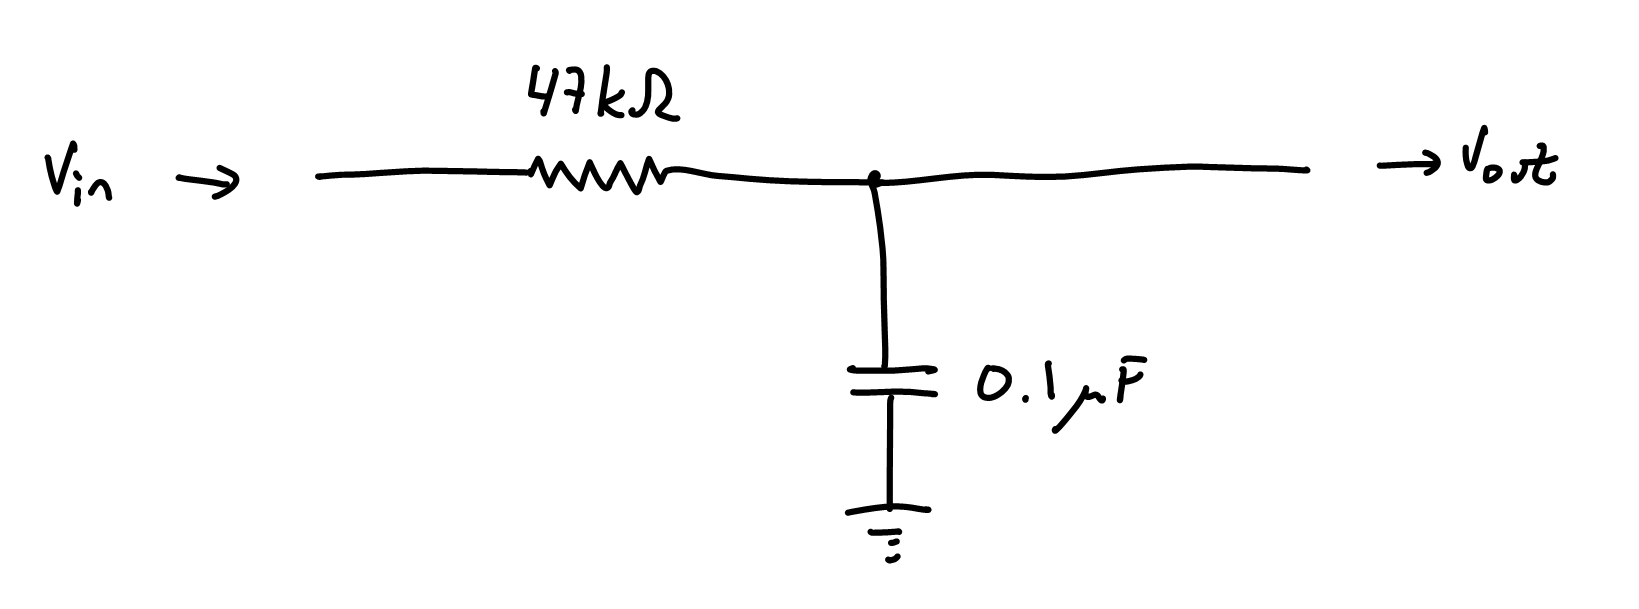
\includegraphics[width=4in]{figures/rc_prelab}
\caption{An RC circuit.}
\label{fig:rc.prelab}
\end{center}
\end{figure}

\item Using a circuit with the same topology, find a resistance, $R$, that gives a rise-time of 1ms if $C=22\mu F$, a common capacitor size. What is the closest \emph{common} resistor you can find?
\vspace{1in}
\item In the oscilloscope image in Figure~\ref{fig:trigger}, what trigger settings are being used (source, condition, and level)?
\vspace{0.75in}

\begin{figure}[htbp]
\begin{center}
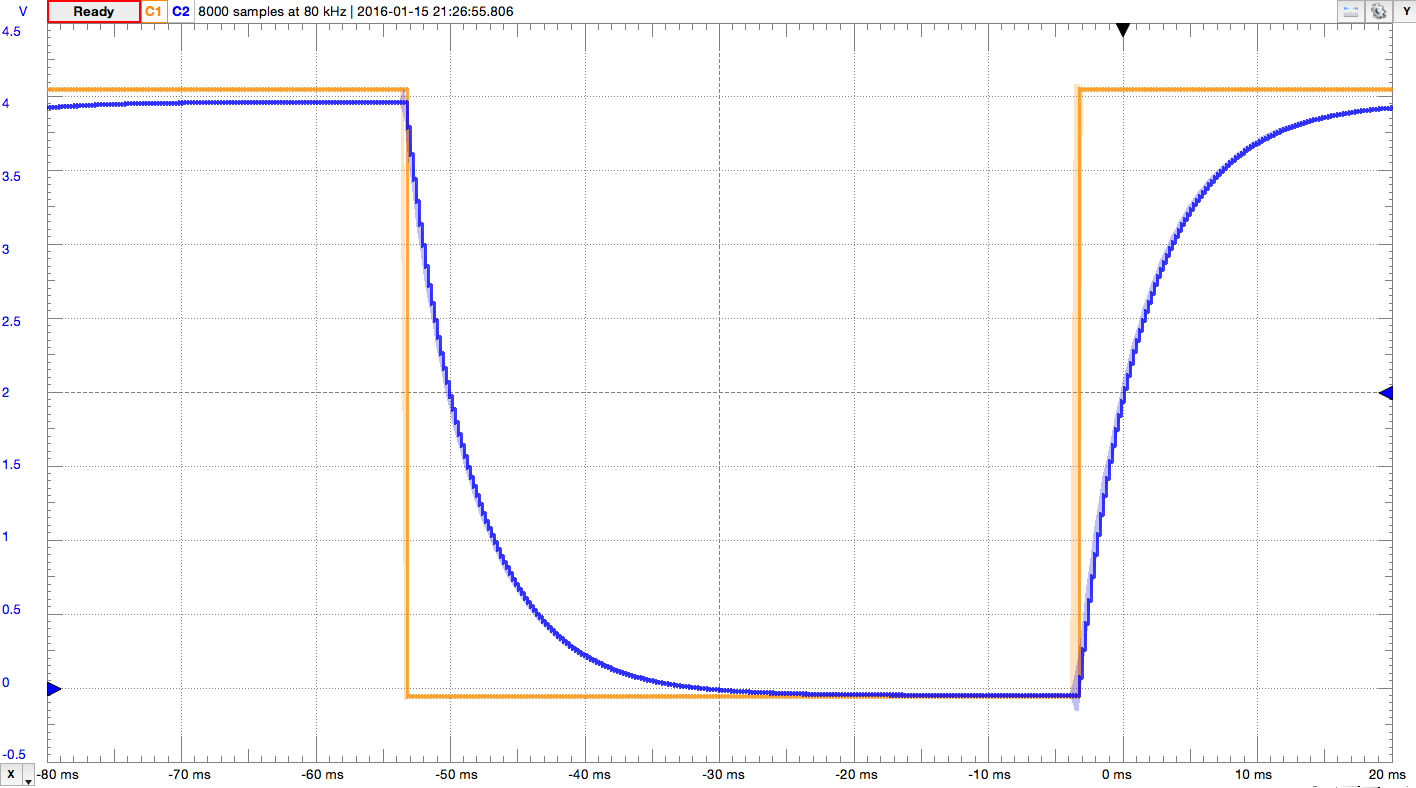
\includegraphics[width=\textwidth]{figures/rc_capture}
\caption{A oscilloscope capture from an RC circuit.}
\label{fig:trigger}
\end{center}
\end{figure}
\end{enumerate}

\end{document}
